\documentclass{beamer}
\usepackage{graphicx}

\title[Bees?]{``Bees?''\\ A Large Scale, Co-operative Simulation Weighing
                          Altruism and Selfishness}
\author{A. Simms, R. Thielstrom}
\institute{Swarthmore College}
\date{Adaptive Robotics, Spring 2014}

\usetheme{Antibes}

\begin{document}

	\begin{frame}
		\titlepage
	\end{frame}

	\section{Overview}

	\begin{frame}{Overview}
		\begin{itemize}
			\item Attempting to investigate conditions for selfishness and altruism in a community of neural-net agents.
			\item Can we get co-operation from a large number of independent agents?
			% \item 
		\end{itemize}
	\end{frame}

	\section{Experiment}

	\begin{frame}{The Bee model}
		\begin{itemize}
			\item Many individual ``bees'' in a ``hive''.
			\item Each bee is an individual NEAT agent.
		\end{itemize}
	\end{frame}

	\begin{frame}{A day in the life of a bee}
		Every ``day'' in the simulation:
		\begin{itemize}
			\item Each bee goes out to get ``nectar''
			\item Has the decision to eat the nectar there, or bring it back to the hive
			\item At the hive, the nectar brought back by the bees is shared equally between the bees that brought back nectar
		\end{itemize}
		Fitness is determined by how much nectar a bee gets in a given day.
	\end{frame}

	\begin{frame}{NEAT Implementation}
		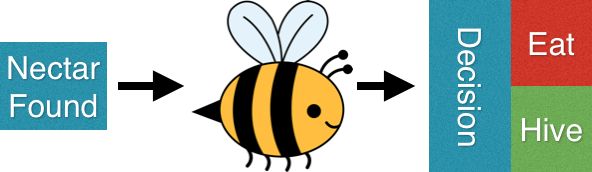
\includegraphics[height=3cm]{bee.png}
	\end{frame}

	\section{Hypothesis}

	\section{Demo}

	\section{Q&A}
	\begin{frame}{Questions?}
		Questions?
	\end{frame}

\end{document}